\chapter{Introduction}

    \section{Background}
        We will first discuss about the key models used for this project.
        
        \subsection{Autoencoders}
            Within unsupervised learning, the study of autoencoders is a very popular field. The most basic form of neural network structure,  takes input vector from the input space $\bm{X}$ and embeds it into the latent space $\bm{Z}$ by the mapping called the \textit{encoder} of the autoencoder. The latent vector is then mapped to the output space $\bm{X'}$ with the same dimension as $\bm{X}$ by the \textit{decoder} of the autoencoder. Finally, this neural network is trained by minimising the $\textit{reconstruction loss}$ between the original input and the final output. Although this idea has been around since 1980s, it has been promoted by \cite{HintonSalakhutdinov2006b}.
            
            \begin{figure}[H] \label{fig:ae}
                \centering
                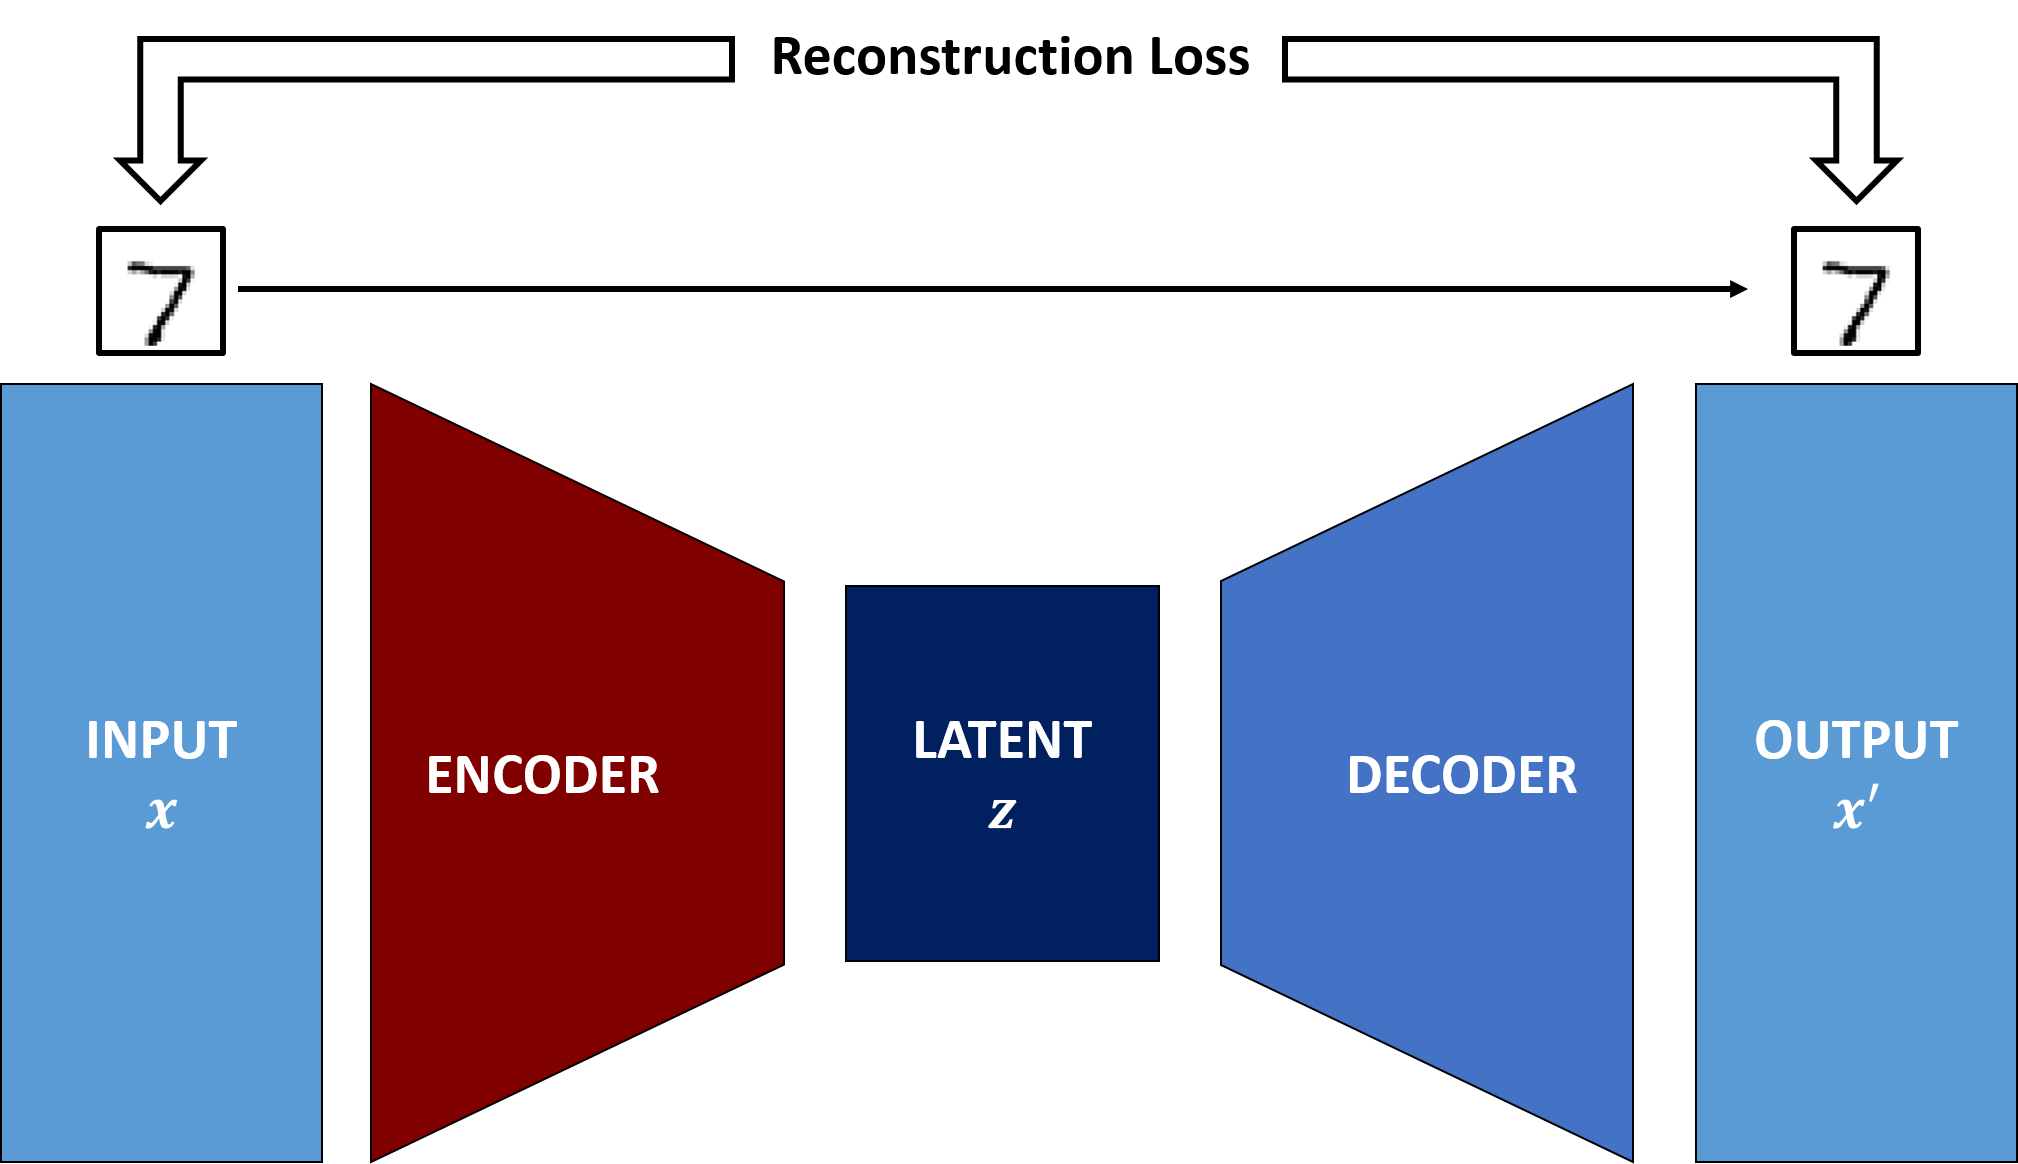
\includegraphics[width=0.5\textwidth]{imgs/autoencoder.png}
                \caption{Basic neural network structure of autoencoders}
            \end{figure}
            
            There are many things autoencoders can achieve even in their basic form. The first is dimensionality reduction. If the dimension of the latent space is chosen to be less than that of the input space, which mostly is the case, then the autoencoder is forced to learn a compressed representation of the input space. Not only does this have immediate practical benefits, for example reducing the file size of images without losing too much quality, it essentially was achieving a form of feature learning.
            
            Another example of what basic autoencoders can do, with a slight modification, is denoising. \cite{vincent2008extracting} proposed a denoising autoencoder which was able to remove noise from an image. This was achieved by first purposefully adding random noise from a fixed distribution to the original image and feeding the noisy image into the autoencoder. Then the autoencoder was trained by minimising the reconstruction loss between the final output image and the original image before adding noise. As well as being able to remove noise from images, it was shown to be a more robust model and had less overfitting than the original autoencoder.
            
            \begin{figure}[H] \label{fig:dae}
                \centering
                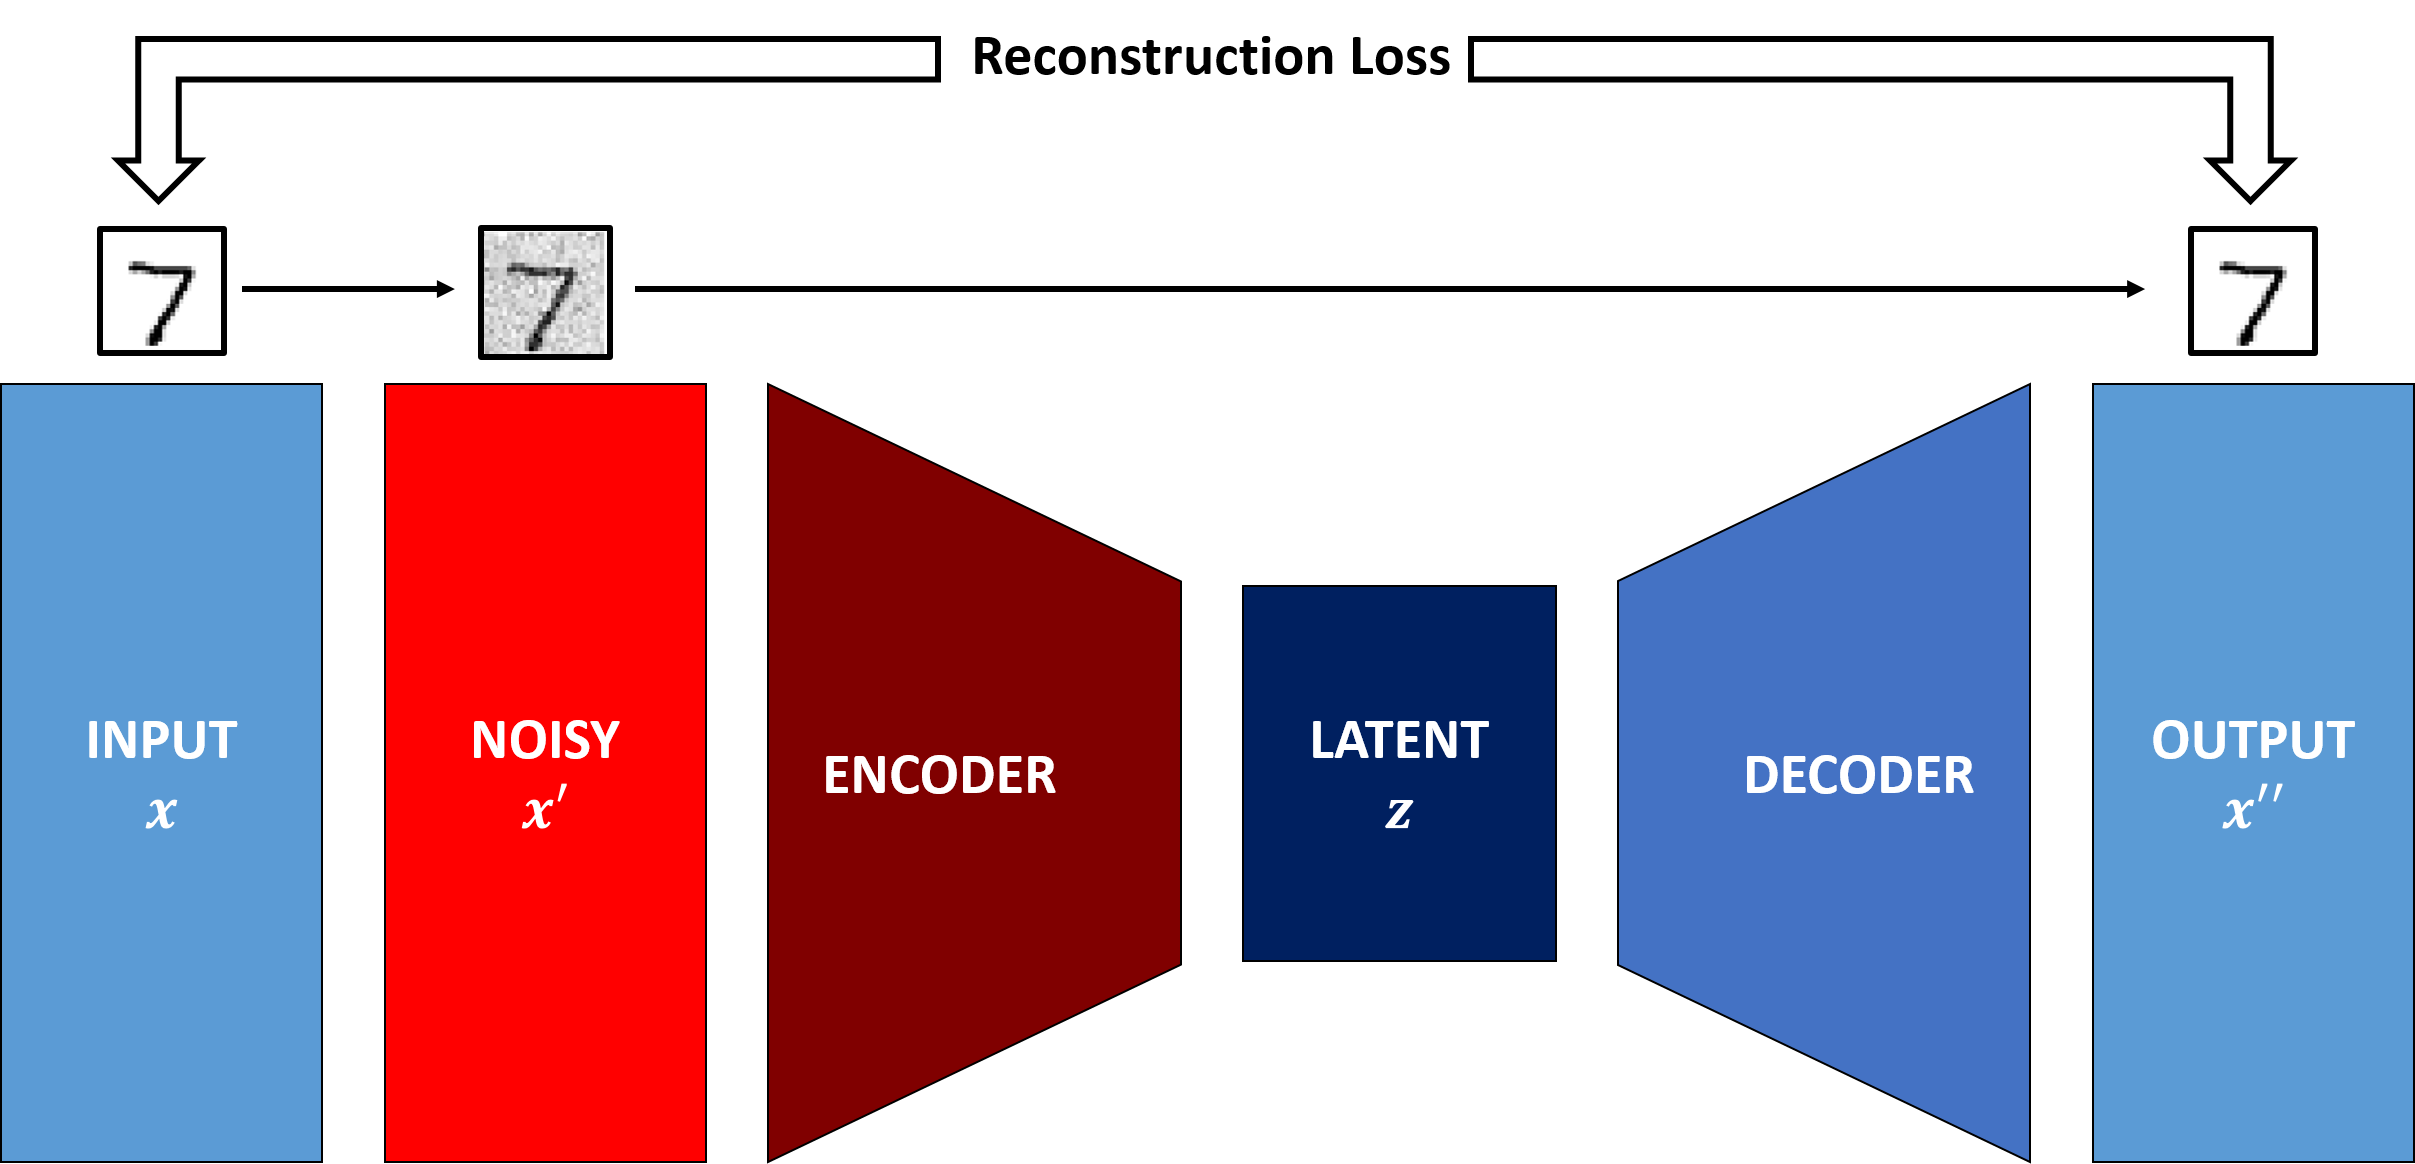
\includegraphics[width=0.5\textwidth]{imgs/denoising_ae.png}
                \caption{Structure of a denoising autoencoder neural network}
            \end{figure}
            
            There were many other further developments on basic autoencoders such as Stacked Denoising Autoencoder \citep{vincent2010stacked}, Contractive Autoencoder \citep{rifai2011higher}, and k-Sparse Autoencoder \citep{makhzani2013k}. These provided further ways of making more robust models that avoids overfitting. However, there is a fundamental limitation to these basic autoencoders which is the limited \textit{interpretability} of the latent space. Of course, this leads us to the question: `What do we mean by \textit{interpretability} of the latent space?'. There are 2 levels of interpretability we will discuss in this project and they are: continuity in the latent space, and disentangled representations. These will be further discussed in the following sections.
            
        \subsection{Variational Autoencoders(VAEs)}
            \subsubsection{Motivation}
                Before going into the details about the VAE\citep{kingma2013auto}, we will first look ahead at what sets this apart from the previous autoencoders in terms of what it can do. As mentioned in the previous section, one limitation of the basic autoencoders is that their latent spaces have poor interpretability. One way in which we can see this is this. Suppose we have a trained model of a basic autoencoder on a set of MNIST images. If we now take two different images of the digit `1' and get the corresponding latent vectors $\bm{z_1}$ and $\bm{z_2}$ using the encoder, what would happen if we take the mean of the two latent vectors, call it $\bm{z_{avg}}$, and feed this vector into the decoder? In many of the basic autoencoders, it is likely to produce an output which doesn't make sense. This is because the autoencoder had not been encouraged to produce a continuous latent space in which the latent vectors in between the learnt latent vectors would interpolate in a meaningful way. Without this encouragement, the latent space is going to be sparse and have many disjoint clusters that represent the original information. An important implication of this limitation is that it is very difficult to generate new images, let alone generating new images with specifiable features.
                
                \begin{figure}[H] \label{fig:int_fail}
                    \centering
                    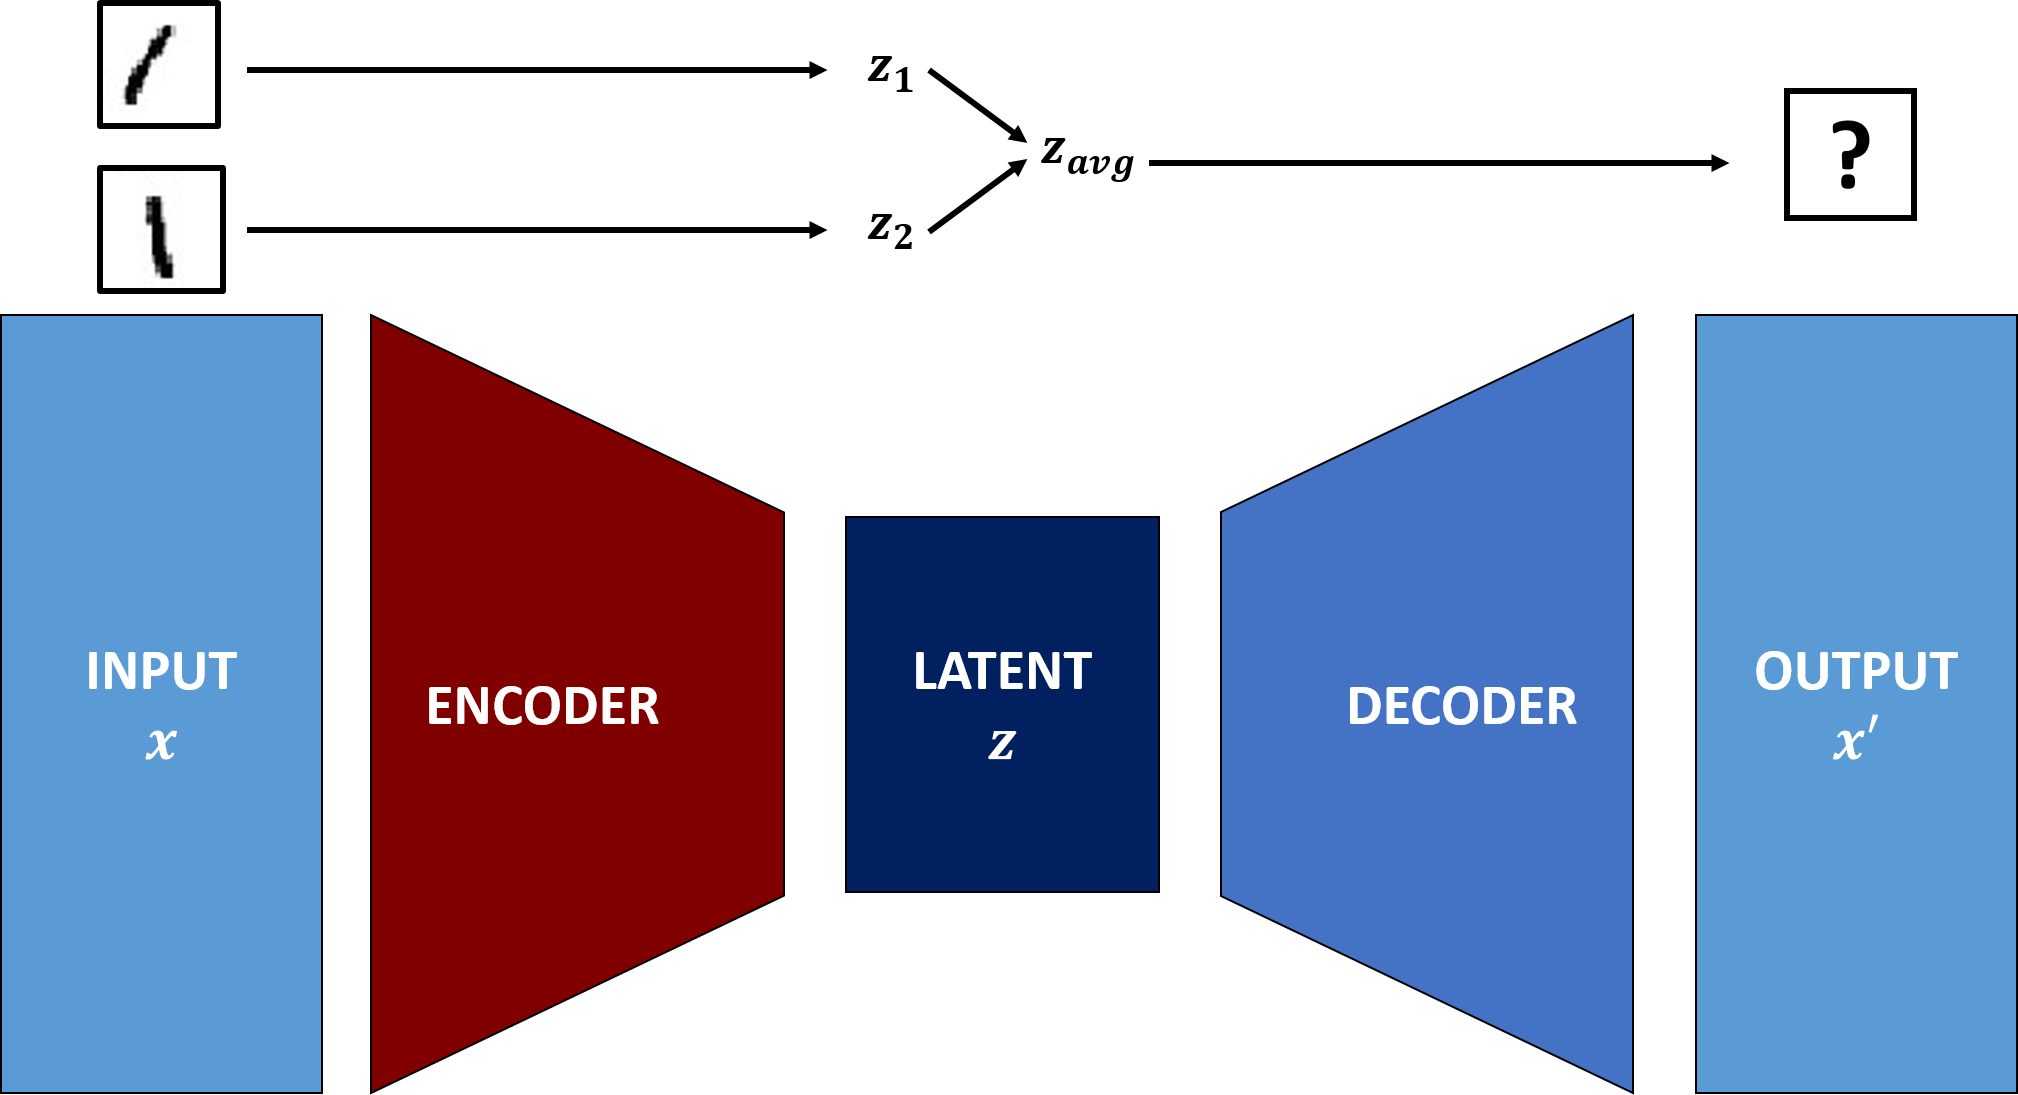
\includegraphics[width=0.5\textwidth]{imgs/interpolation_fail.png}
                    \caption{Basic autoencoders have difficulty with interpolation}
                \end{figure}
                
                On the other hand, VAEs produces a continuous latent space in which the interpolation between the latent vectors represent a much better interpolation between the original vectors. We will now discuss the theory behind the VAEs which makes this possible.
                
            \subsubsection{High level explanation of VAE}
                VAE takes an input data point $\bm{x}$ and passes it through an encoder just like normal autoencoders. However, instead of mapping the input data point as a latent data point, it maps it as a probability distribution $ENCODER(\bm{x}) \rightarrow q_{\bm{\theta_x}}(\bm{z}|\bm{x})$, where $\bm{\theta_x}$ is the parameter vector defining the distribution $q$. The standard distribution for the VAE's latent space is the uncorrelated multivariate Gaussian distribution $\mathcal{N}(\bm{\mu}, \bm{\Sigma})$ where $\bm{\Sigma}$ is a diagonal covariance matrix. So $\bm{\theta_x} = \{\bm{\mu_x}, \bm{\Sigma_x}\}$ and since $\bm{\Sigma_x}$ is diagonal, the mean $\mu_{x_i}$ and variance $\sigma_{x_i}^2$ in each dimension are all the parameters required to describe the distribution. This is the key which makes the meaningful continuous latent space possible as the VAE's latent space is composed of continuously overlapping distributions. From this distribution $q_{\bm{\theta_x}}(\bm{z}|\bm{x})$, a single latent vector is sampled at random $\bm{z'} \sim q_{\bm{\theta_x}}(\bm{z}|\bm{x})$ which is then fed into the decoder to construct the output vector $DECODER(\bm{z'}) \rightarrow \bm{x'}$.
                
                \begin{figure}[H] \label{fig:vae_arch}
                    \centering
                    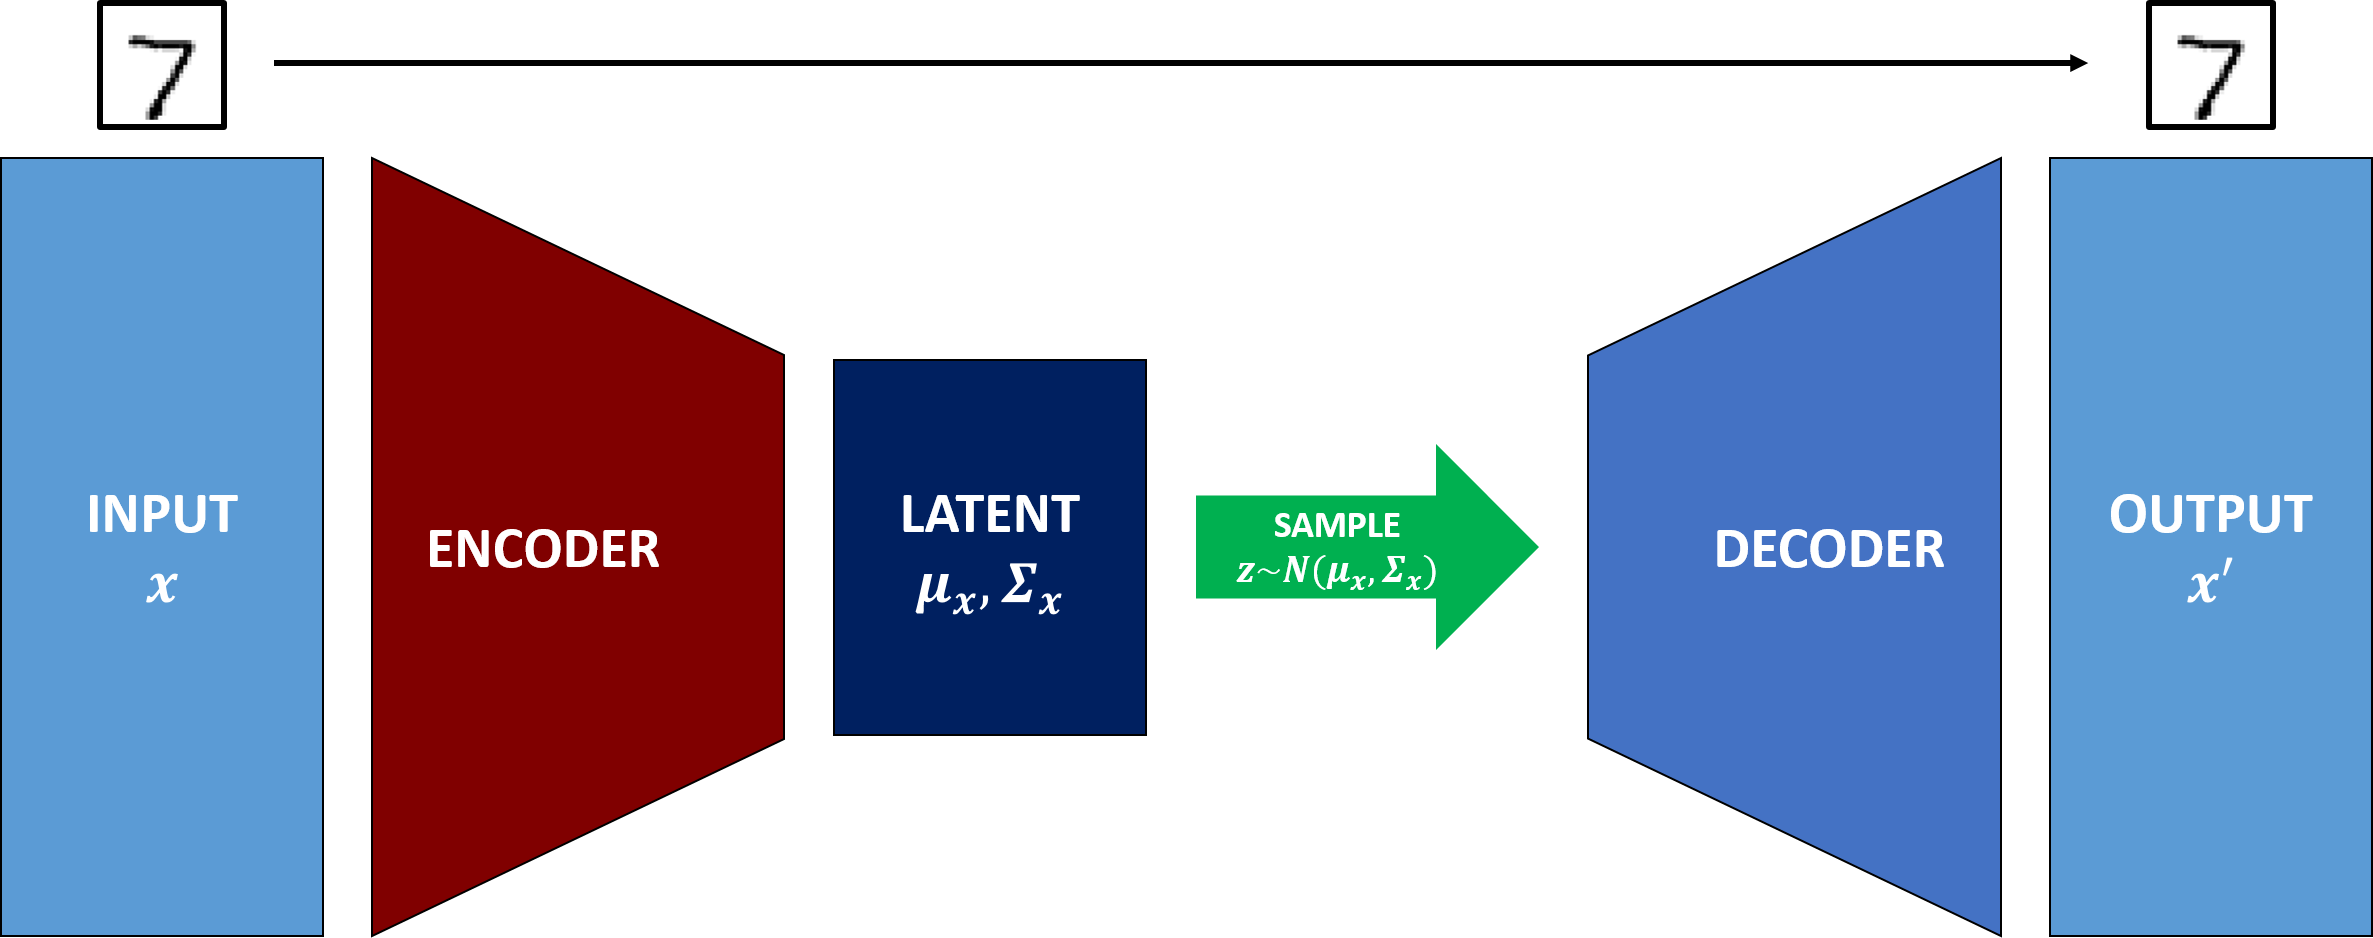
\includegraphics[width=0.5\textwidth]{imgs/vae_arch.png}
                    \caption{VAE's architecture}
                \end{figure}

                When training a VAE, the process is slightly more involved. Firstly, since the latents are distributions as opposed to single points, we cannot calculate the reconstruction loss in the same way as with basic autoencoders. What should the model compare the original input to? One possible candidate is the output of the mean of the encoded distribution. However, this approach will not be able to take the variance of the distribution into account. Another candidate is the output of a randomly sampled point from the encoded distribution. Unfortunately, a single point is insufficient to convey the information of the whole distribution. What we need is to take a large enough sample from the distribution and take the expectation of the reconstruction losses between the original input and the sampled outputs.
                
                \begin{figure}[H] \label{fig:recon_loss}
                    \centering
                    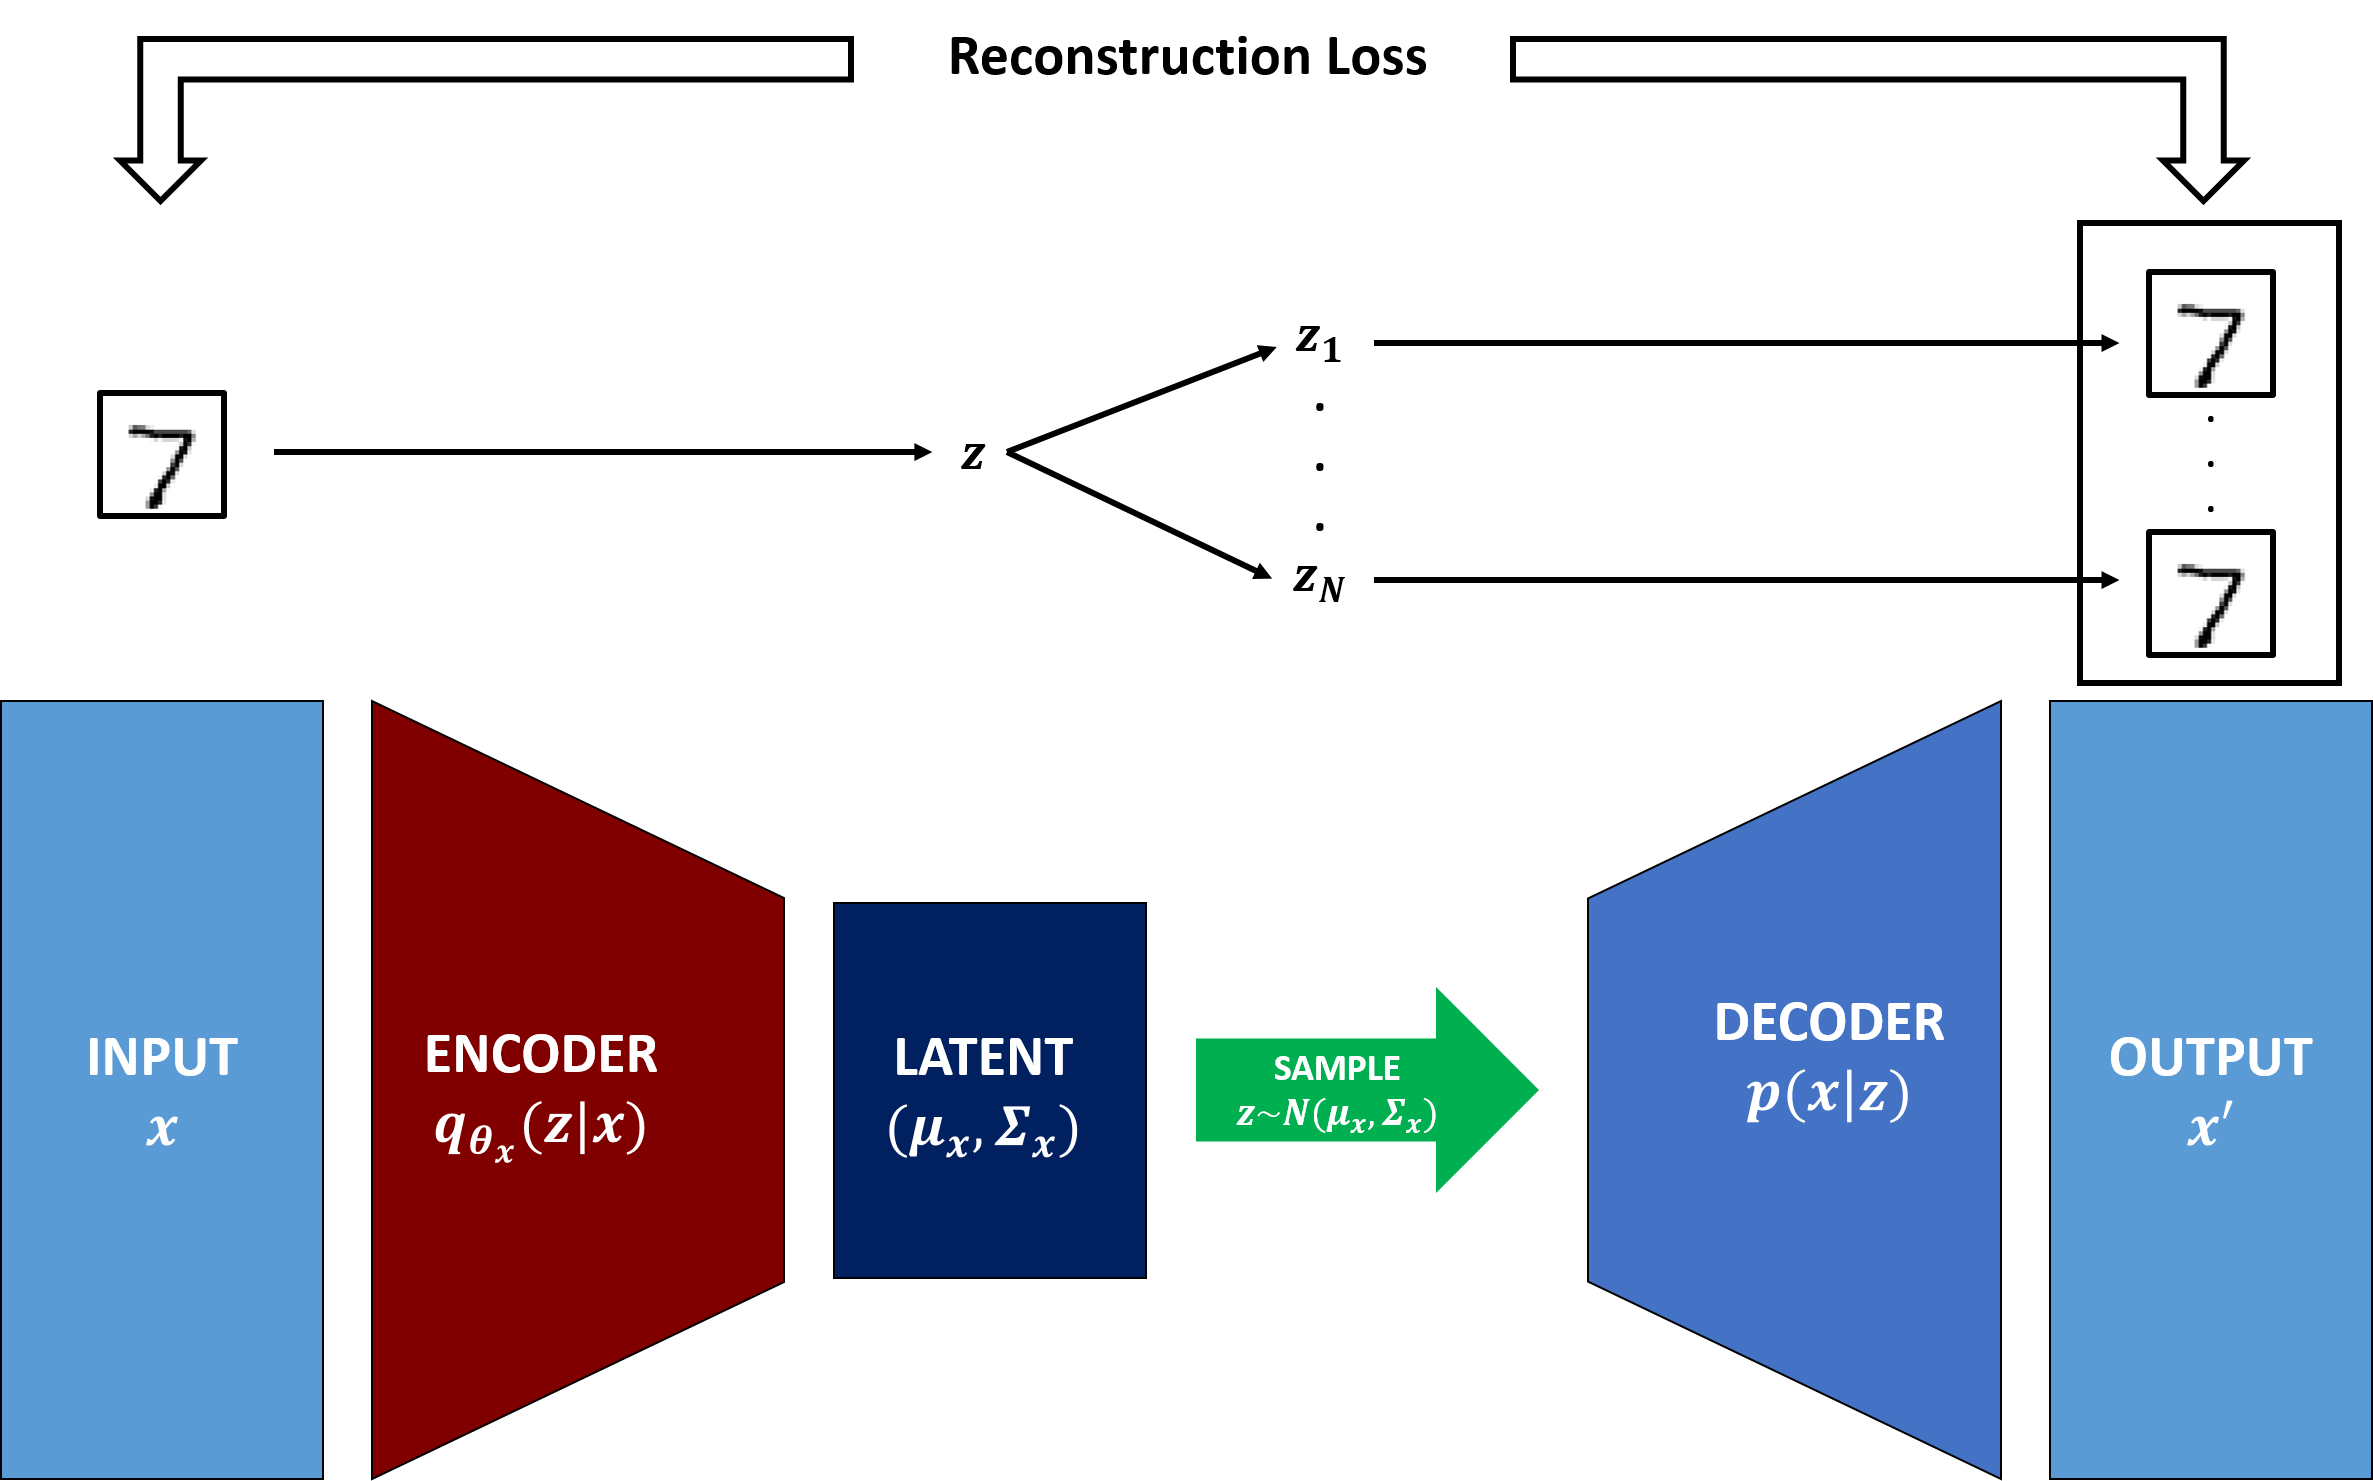
\includegraphics[width=0.5\textwidth]{imgs/recon_loss.png}
                    \caption{VAE's reconstruction loss}
                \end{figure}
                
                So far, what we have is a model which will learn to best represent the input space by modelling the latent space with Gaussian distributions. The problem at this stage is a form of overfitting. This is because nothing is stopping the model to make use of all of the dimensions in the latent space and to produce many disjoint Gaussians with very small variances which could almost become a representation of a point. This overfitting can especially become a problem if the dimension of the latent space is much larger than the number of features present in the input space. The consequence of this overfitting is that we don't really get a continuous latent space. Instead, we get disjoint clusters which vary across the various dimensions. This is a form of the classic problem in machine learning of overfitting due to having too much degree of freedom of model complexity. The answer is to apply the standard remedy: a regulariser. We need a choice of a regulariser which penalises the model for making use of more and more dimensions in the latent space to represent the input space and the Kullback–Leibler divergence \citep{kullback1951information}(KL divergence) is used to do this. The exact mathematical definition and the derivation of the KL divergence's appearance in the loss function is discussed below, but for now, we will simply explain what effect the KL divergence has on the model. KL divergence is like a metric which measures the difference between two probability distributions. With this, we will measure the difference between $q_{\bm{\theta}}(\bm{z}|\bm{x}_{in})$ and $p(\bm{z})$ where $p(\bm{z})$ is the standard Gaussian distribution $\mathcal{N}(\bm{0}, \bm{I})$. Now if we add this KL divergence term to our loss, the model is pushed to keep the shape of $q_{\bm{\theta}}(\bm{z}|\bm{x}_{in})$ not too far from the standard Gaussian, otherwise KL divergence will become large and incur a large loss. This has two main implications. First, VAE will try to keep as much latent dimensions to have standard Gaussian parameters which leads to using least number of latent dimensions as possible. Secondly, VAE will be penalised when it tries to use small standard deviations to try and make small size clusters. This means that VAE is encouraged to make larger cluster of close data points together so that hopefully, closer data points in the input space are mapped into the same distribution.
                
                \begin{figure}[H] \label{fig:kl_effect}
                    \centering
                    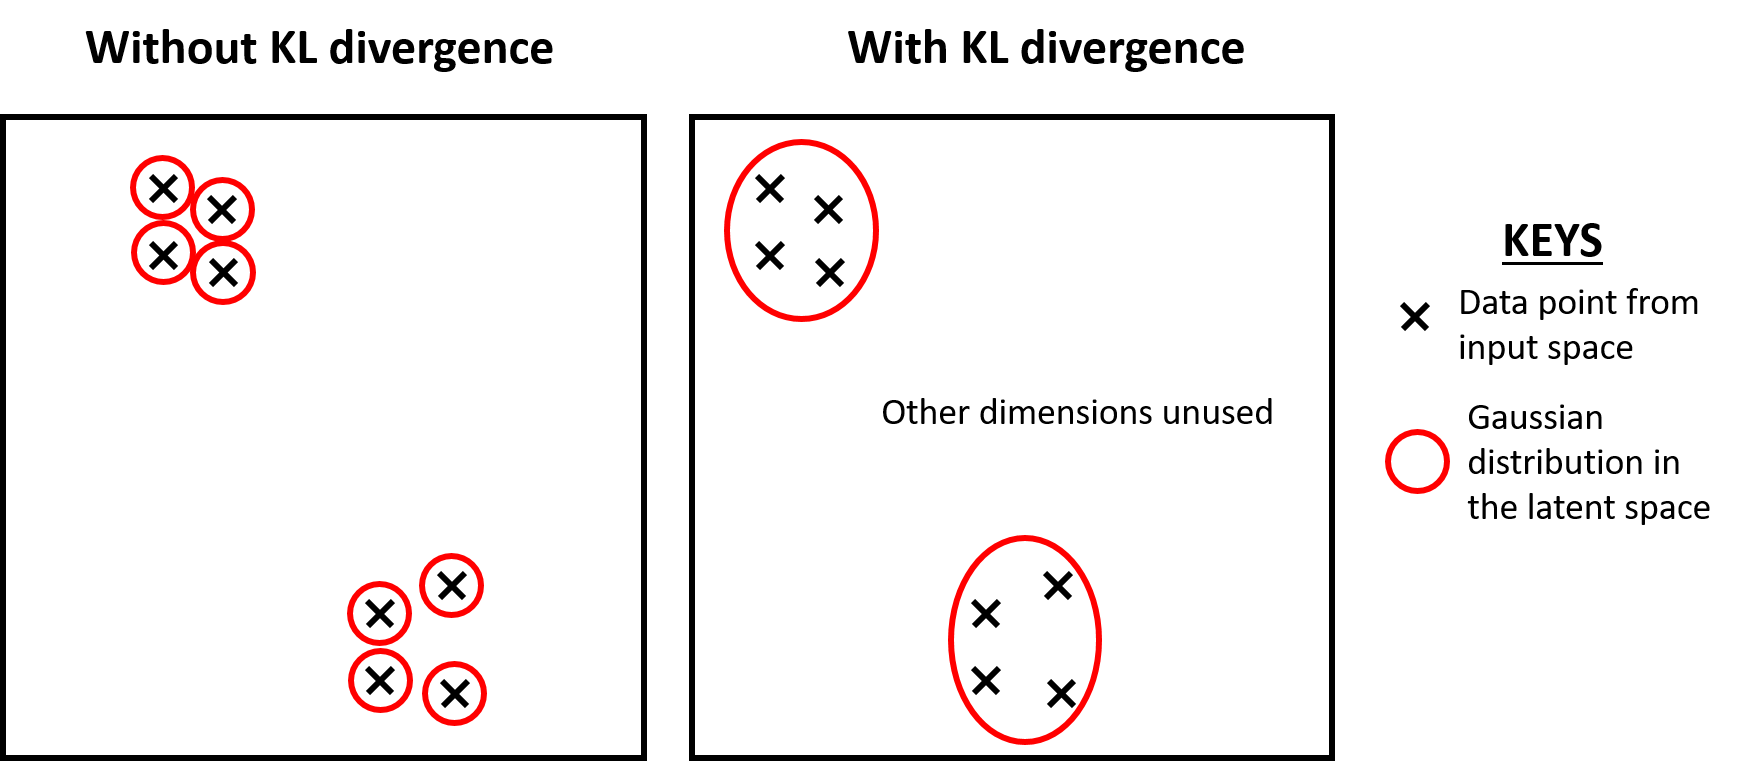
\includegraphics[width=0.5\textwidth]{imgs/kl_effect.png}
                    \caption{The effect of KL divergence}
                \end{figure}
                
                In summary, VAE is trained with the sum of the reconstruction loss, which is the expectation of the differences between the original input data and the samples of output data, together with the KL divergence between the latent uncorrelated Gaussian distribution and the standard Gaussian distribution:
                \begin{equation} \label{eqn:loss_vae}
                    \text{Loss\textsubscript{VAE}} = \text{Reconstruction Loss} + \text{KL Divergence}
                \end{equation}
                
            \subsubsection{Probabilistic descriptions and mathematical derivations}
                We start with the observed space $\bm{X}$ composed of data points $\bm{x}$. We begin with an assumption that the each $\bm{x}$ are independently and identically distributed(iid) by some probability function of some corresponding latent variables $\bm{z}$ which are unobserved or hidden. Let $p(\bm{x}|\bm{z})$ be the probability of observing $\bm{x}$ given the latent $\bm{z}$, also known as the \textit{likelihood} function. We also assume that each latent $\bm{z}$ are distributed with some function which we denote by $p(\bm{z})$, also known as the \textit{prior}. The relationship can be illustrated with the following graphical model:
                
                \begin{figure}[H] \label{fig:x_z_graph}
                    \centering
                    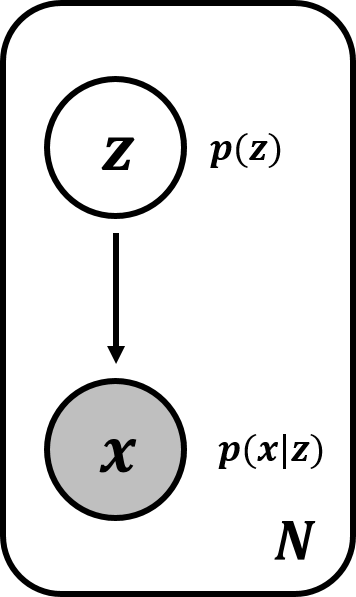
\includegraphics[width=0.15\textwidth]{imgs/x_z_graph.png}
                    \caption{The graphical model showing the relationship between $\bm{x}$ and $\bm{z}$}
                \end{figure}
                
                Now given the prior and the likelihood, we can use the classical Bayes' theorem to express the \textit{posterior}:
                
                \begin{align*} 
                    p(\bm{z}|\bm{x}) &= \frac{p(\bm{z},\bm{x})}{p(\bm{x})}\\
                    &= \frac{p(\bm{x} | \bm{z})p(\bm{z})}{p(\bm{x})}\\
                    &= \frac{p(\bm{x} | \bm{z})p(\bm{z})}{\int p(\bm{x}, \bm{z}) dz}\\
                    &= \frac{p(\bm{x} | \bm{z})p(\bm{z})}{\int p(\bm{x} | \bm{z}) p(\bm{z}) dz}\\
                \end{align*}

                Unfortunately, the term which appears in the denominator of the posterior: $p(\bm{x}) = \int p(\bm{x} | \bm{z}) p(\bm{z}) dz$, is intractable as the integral requires exponential computational time to calculate over all the possible values of the latents. Because of this problem of intractable posterior, VAE instead uses a family of tractable functions $q_{\bm{\theta_x}}(\bm{z}|\bm{x})$ which best \textit{approximates} the true posterior $p(\bm{z}|\bm{x})$. Notice that the family of functions are parametrised by $\bm{\theta_x}$ which in turn depends on the input $\bm{x}$. In the standard VAE, $q_{\bm{\theta}}(\bm{z}|\bm{x})$ are chosen to be Gaussians which means that $\bm{\theta_x}= \{\bm{\mu_x}, \bm{\Sigma_x}\}$.
                
                Now in order to make sure that $q_{\bm{\theta_x}}(\bm{z}|\bm{x})$ closely approximates $p(\bm{z}|\bm{x})$, we can minimise:
                    \[ KL\left[q_{\bm{\theta_x}}(\bm{z}|\bm{x}) || p(\bm{z}|\bm{x})\right] \]
                where the $KL\left[q(\bm{x}) || p(\bm{x})\right]$ is the Kullback-Leibler(KL) divergence, measuring the difference between the two distributions, defined by:
                    \[ KL\left[q(\bm{x}) || p(\bm{x})\right] := \int_{\bm{x} \in \bm{X}} q(\bm{x}) \log \frac{q(\bm{x})}{p(\bm{x})} d\bm{x}\]
                In other words, we wish to minimise:
                    \[ KL\left[q_{\bm{\theta_x}}(\bm{z}|\bm{x}) || p(\bm{z}|\bm{x})\right] = \int_{\bm{z} \in \bm{Z}} q_{\bm{\theta_x}}(\bm{z}|\bm{x}) \log \frac{q_{\bm{\theta_x}}(\bm{z}|\bm{x})}{p(\bm{z}|\bm{x})} d\bm{z}\]
                
                The problem is not yet solved as the term still includes the intractable posterior $p(\bm{z}|\bm{x})$. To address this problem, we will minimise the KL divergence indirectly by using what's known as the \textit{Evidence Lower BOund}($ELBO$):
                    \[ ELBO(\bm{\theta_x}) := \log p(\bm{x}) - KL\left[q_{\bm{\theta_x}}(\bm{z}|\bm{x}) || p(\bm{z}|\bm{x})\right] \]
                Keeping all other parameters fixed, we can see that maximising $ELBO$ with respect to $\bm{\theta_x}$ minimises the KL divergence since the KL divergence is non-negative due to Jensen's inequality\citep{jensen1906fonctions}. Doing some algebraic manipulation removes both intractable terms $p(\bm{x})$ and $p(\bm{z}|\bm{x})$ in the equation. We first begin by manipulating $\log p(\bm{x})$:
                
                \begin{align*}
                  \log p(\bm{x}) &= \log p(\bm{x}) \int_{\bm{z} \in \bm{Z}} q_{\bm{\theta_x}}(\bm{z}|\bm{x}) d\bm{z} & \text{$q$ is a probability density function}\\
                    &= \int_{\bm{z} \in \bm{Z}} q_{\bm{\theta_x}}(\bm{z}|\bm{x}) \log p(\bm{x}) d\bm{z} & \text{$\bm{z}$ does not appear in $\log p(\bm{x})$}\\
                    &= \int_{\bm{z} \in \bm{Z}} q_{\bm{\theta_x}}(\bm{z}|\bm{x}) \log \frac{p(\bm{x}, \bm{z})}{p(\bm{z} | \bm{x})} d\bm{z} & \text{Using $p(\bm{z} | \bm{x}) = \frac{p(\bm{x}, \bm{z})}{p(\bm{x})}$}\\
                    &= \int_{\bm{z} \in \bm{Z}} q_{\bm{\theta_x}}(\bm{z}|\bm{x}) \log \frac{p(\bm{x}, \bm{z})}{q_{\bm{\theta_x}}(\bm{z}|\bm{x})}\frac{q_{\bm{\theta_x}}(\bm{z}|\bm{x})}{p(\bm{z} | \bm{x})} d\bm{z} & \frac{q_{\bm{\theta_x}}(\bm{z}|\bm{x})}{q_{\bm{\theta_x}}(\bm{z}|\bm{x})} = 1\\
                    &= \int_{\bm{z} \in \bm{Z}} q_{\bm{\theta_x}}(\bm{z}|\bm{x}) \log \frac{p(\bm{x}, \bm{z})}{q_{\bm{\theta_x}}(\bm{z}|\bm{x})} + q_{\bm{\theta_x}}(\bm{z}|\bm{x}) \log \frac{q_{\bm{\theta_x}}(\bm{z}|\bm{x})}{p(\bm{z} | \bm{x})} d\bm{z} & \text{$\log$ property}\\
                    &= \int_{\bm{z} \in \bm{Z}} q_{\bm{\theta_x}}(\bm{z}|\bm{x}) \log \frac{p(\bm{x}, \bm{z})}{q_{\bm{\theta_x}}(\bm{z}|\bm{x})} d\bm{z} + \int_{\bm{z} \in \bm{Z}} q_{\bm{\theta_x}}(\bm{z}|\bm{x}) \log \frac{q_{\bm{\theta_x}}(\bm{z}|\bm{x})}{p(\bm{z} | \bm{x})} d\bm{z} & \text{Linearity of integrals}\\
                    &= \int_{\bm{z} \in \bm{Z}} q_{\bm{\theta_x}}(\bm{z}|\bm{x}) \log \frac{p(\bm{x}, \bm{z})}{q_{\bm{\theta_x}}(\bm{z}|\bm{x})}d\bm{z} + KL\left[q_{\bm{\theta_x}}(\bm{z}|\bm{x}) || p(\bm{z}|\bm{x})\right] & \text{Definition of $KL$}\\
                \end{align*}
                
                Therefore, substituting the final form back into $ELBO$, we get:
                
                \begin{align*}
                    ELBO(\bm{\theta_x}) &= \log p(\bm{x}) - KL\left[q_{\bm{\theta_x}}(\bm{z}|\bm{x}) || p(\bm{z}|\bm{x})\right]\\
                    &= \int_{\bm{z} \in \bm{Z}} q_{\bm{\theta_x}}(\bm{z}|\bm{x}) \log \frac{p(\bm{x}, \bm{z})}{q_{\bm{\theta_x}}(\bm{z}|\bm{x})} d\bm{z} + KL\left[q_{\bm{\theta_x}}(\bm{z}|\bm{x}) || p(\bm{z}|\bm{x})\right] - KL\left[q_{\bm{\theta_x}}(\bm{z}|\bm{x}) || p(\bm{z}|\bm{x})\right]\\
                    &= \int_{\bm{z} \in \bm{Z}} q_{\bm{\theta_x}}(\bm{z}|\bm{x}) \log \frac{p(\bm{x}, \bm{z})}{q_{\bm{\theta_x}}(\bm{z}|\bm{x})} d\bm{z}\\
                    &= \int_{\bm{z} \in \bm{Z}} q_{\bm{\theta_x}}(\bm{z}|\bm{x}) \log \frac{p(\bm{x} | \bm{z})p(\bm{z})}{q_{\bm{\theta_x}}(\bm{z}|\bm{x})} d\bm{z}\\
                    &= \int_{\bm{z} \in \bm{Z}} q_{\bm{\theta_x}}(\bm{z}|\bm{x}) \log p(\bm{x} | \bm{z}) + q_{\bm{\theta_x}}(\bm{z}|\bm{x}) \log \frac{p(\bm{z})}{q_{\bm{\theta_x}}(\bm{z}|\bm{x})} d\bm{z}\\
                    &= \int_{\bm{z} \in \bm{Z}} q_{\bm{\theta_x}}(\bm{z}|\bm{x}) \log p(\bm{x} | \bm{z}) d\bm{z} + \int_{\bm{z} \in \bm{Z}} q_{\bm{\theta_x}}(\bm{z}|\bm{x}) \log \frac{p(\bm{z})}{q_{\bm{\theta_x}}(\bm{z}|\bm{x})} d\bm{z}\\
                    &= \mathbb{E}_{q_{\bm{\theta_x}}(\bm{z}|\bm{x})} \left[\log p(\bm{x} | \bm{z}) \right] + KL\left[q_{\bm{\theta_x}}(\bm{z}|\bm{x}) || p(\bm{z})\right]\\
                \end{align*}
                
                As claimed above, all terms in this expression are tractable and so we can use $ELBO$ as our loss function. We also notice that this is exactly what we had in \ref{eqn:loss_vae}:
                
                \[ \boxed{\text{Loss\textsubscript{VAE}} = \underbrace{\mathbb{E}_{q_{\bm{\theta_x}}(\bm{z}|\bm{x})} \left[\log p(\bm{x} | \bm{z}) \right]}_\textrm{Reconstruction Loss} + \underbrace{KL\left[q_{\bm{\theta_x}}(\bm{z}|\bm{x}) || p(\bm{z})\right]}_\textrm{KL Divergence}} \]
                
            \subsubsection{The reparametrisation trick}
                There is one last difficulty that must be addressed in implementing the VAE as a neural network. In \ref{fig:vae_arch}, one of the operation in the network is sampling from the latent distribution:
                
                \begin{figure}[H] \label{fig:sampling}
                    \centering
                    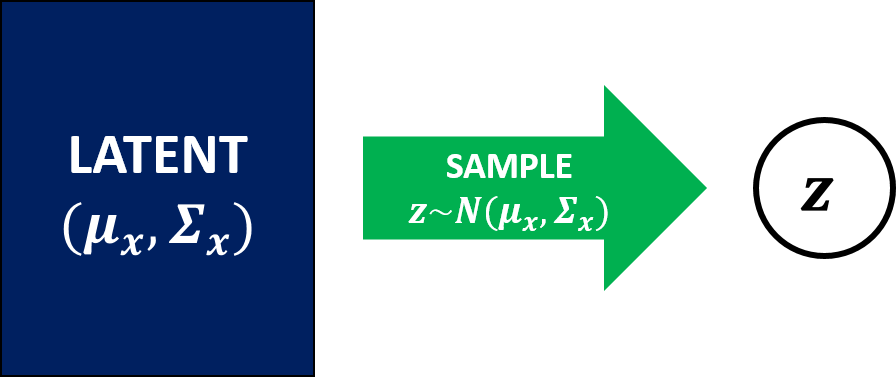
\includegraphics[width=0.4\textwidth]{imgs/sampling.png}
                    \caption{We cannot back propagate through sampling}
                \end{figure}
                
                Unfortunately, sampling is not an operation in which we can take the gradient for back propagation. To deal with this problem, \cite{kingma2013auto} takes advantage of the fact that the covariance $\bm{\Sigma_x}$ is a diagonal matrix and use a technique called \textit{the reparametrisation trick} in which we arrive at the sampled latent $\bm{z}$ not directly from the latent Gaussian distribution, but indirectly by sampling a noise vector from a standard Gaussian distribution and then arriving at the latent $\bm{z}$ by scaling it by $\bm{\Sigma_x}$ and by translating it by $\bm{\mu_x}$. This has the same output as sampling directly from the latent distribution but now at least we can take the separate gradient through $\frac{\partial \bm{z}}{\partial \bm{\mu_x}}$ and $\frac{\partial \bm{z}}{\partial \bm{\Sigma_x}}$:
                
                \begin{figure}[H] \label{fig:reparametrisation_trick}
                    \centering
                    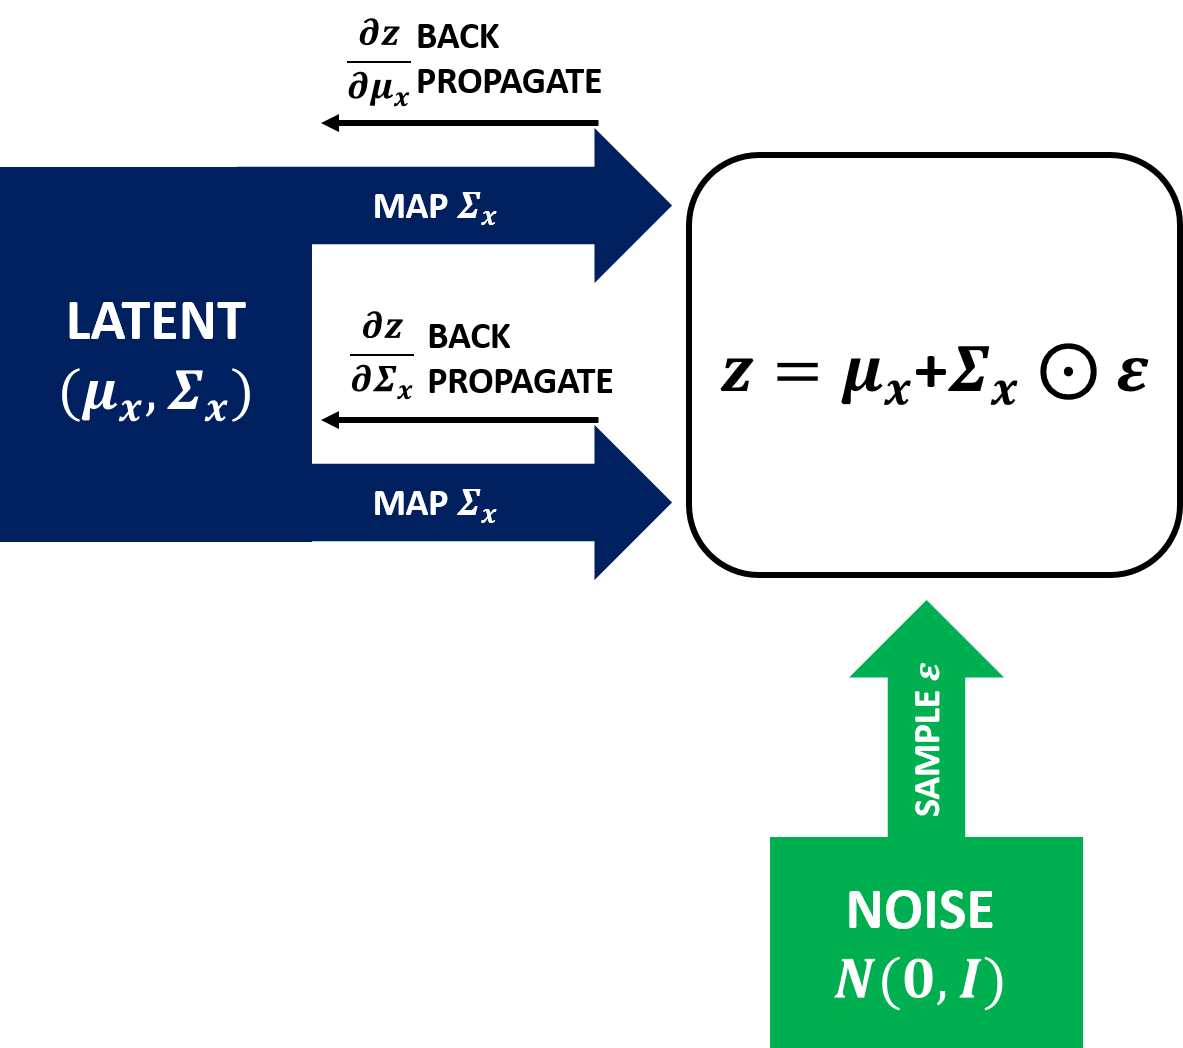
\includegraphics[width=0.4\textwidth]{imgs/reparametrisation_trick.png}
                    \caption{The reparametrisation trick}
                \end{figure}
                
                So the actual full architecture of VAE is the following.
                
                \begin{figure}[H] \label{fig:vae_arch2}
                    \centering
                    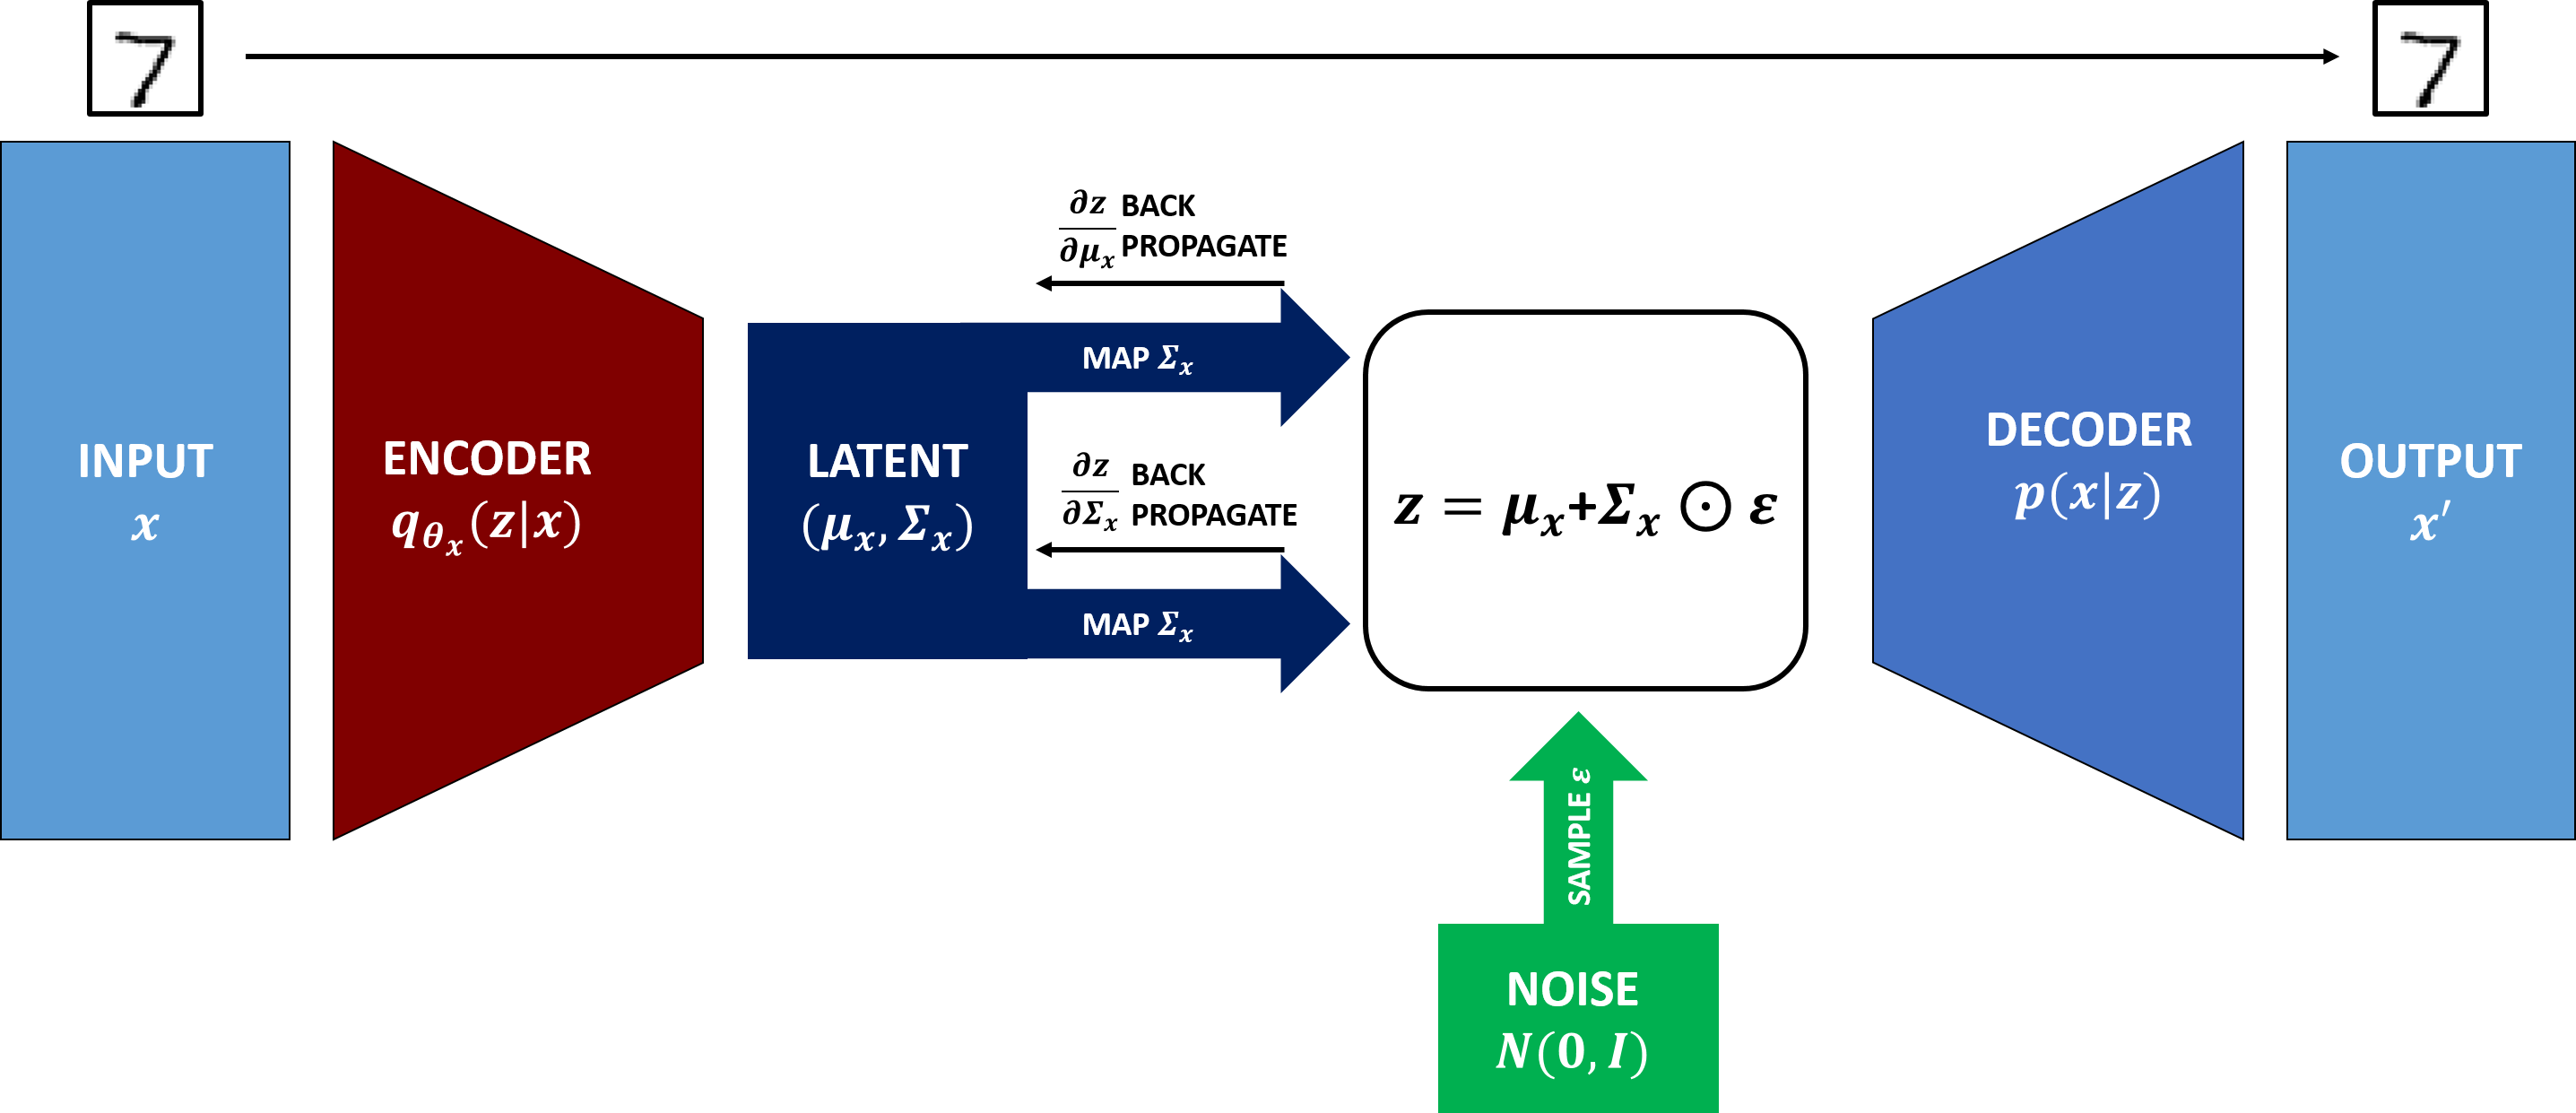
\includegraphics[width=1\textwidth]{imgs/vae_arch2.png}
                    \caption{The full VAE architecture}
                \end{figure}
                
            \subsubsection{Outputs}
                \cite{kingma2013auto} already showed that VAE produces latent spaces which satisfy our first condition of interpretability very well: it produces a continuous latent space in which locality in the input space is preserved in the latent space which allows for great interpolations between data points.
                
                \begin{figure}[H] \label{fig:vae_freyface_mnist}
                    \centering
                    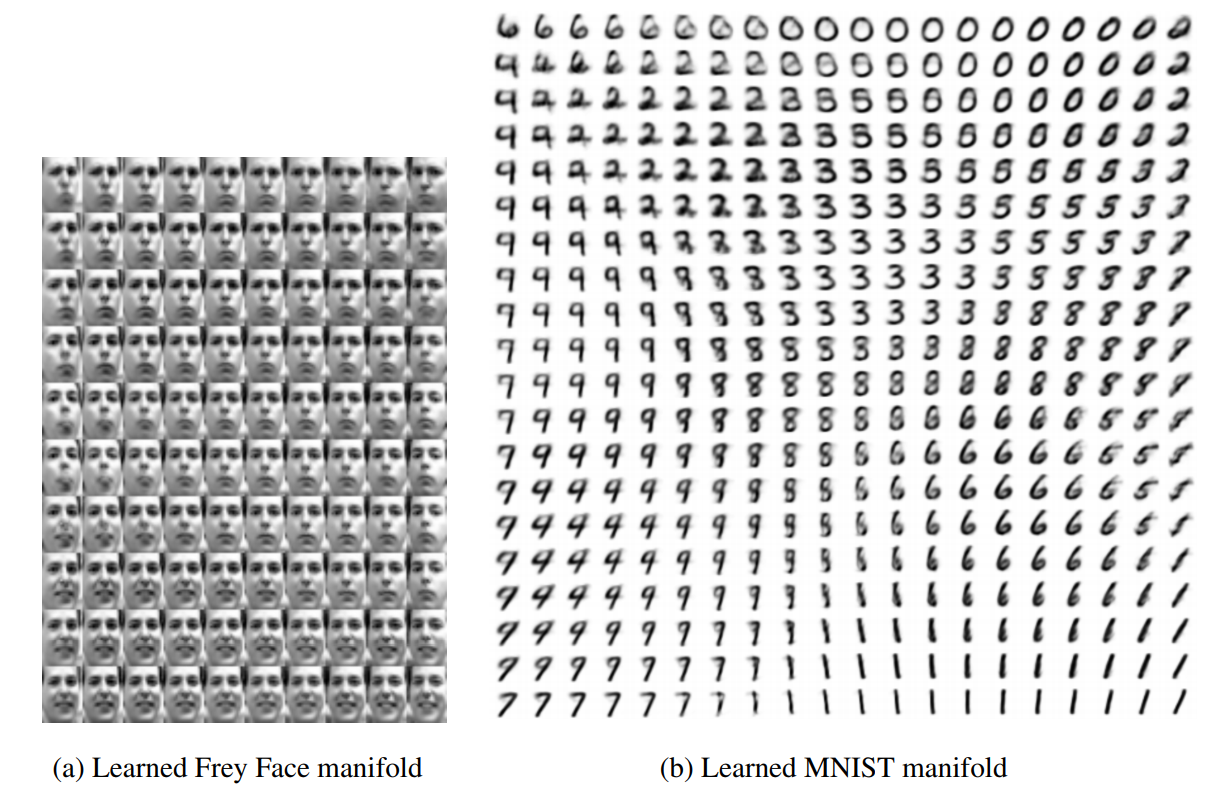
\includegraphics[width=1\textwidth]{imgs/vae_freyface_mnist.png}
                    \caption{Figure by \cite{kingma2013auto} which shows the generated images from the latent values traversed uniformly across the 2D latent space.}
                \end{figure}

                As we can see in the figure \ref{fig:vae_freyface_mnist}, the interpolated images between the images are continuous and make sense. If we consider the MNIST generated images, we even have interpolations between 2 different digits which seem almost plausible.
                
                In fact, VAE also does well at producing latent spaces which satisfy the second condition of interpretability: disentangled representations. \cite{bengio2013representation} defined disentangled representation to have the property such that changes in the single latent dimension changes a single generative factor whilst leaving other generative factors unchanged. \cite{higgins2016beta} includes figures showing how much VAE's representations are disentangled compared so other models which also achieves disentangled representations:
                
                \begin{figure}[H] \label{fig:celeba}
                    \centering
                    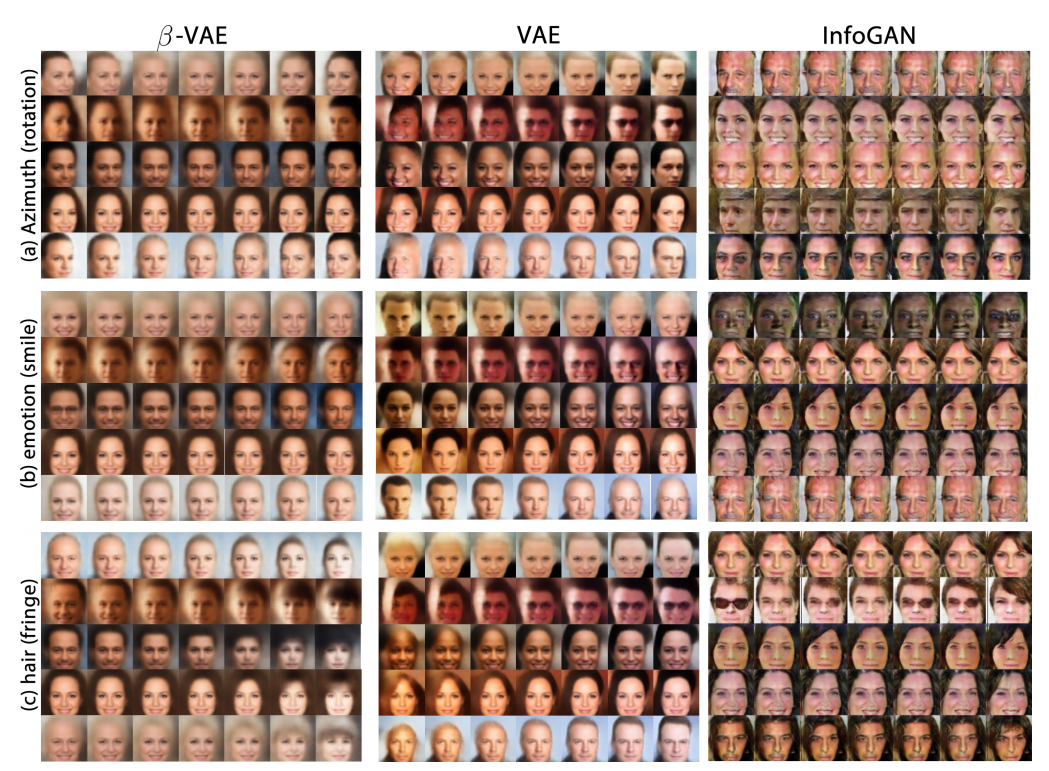
\includegraphics[width=1\textwidth]{imgs/celeba.png}
                    \caption{Figures from \cite{higgins2016beta}. Qualitative comparison on disentanglement between $\beta$-VAE\citep{higgins2016beta}, VAE\citep{kingma2014adam}, and InfoGAN\citep{chen2016infogan} on images of celebrity faces.}
                \end{figure}    
                
                \begin{figure}[H] \label{fig:3d_chairs}
                    \centering
                    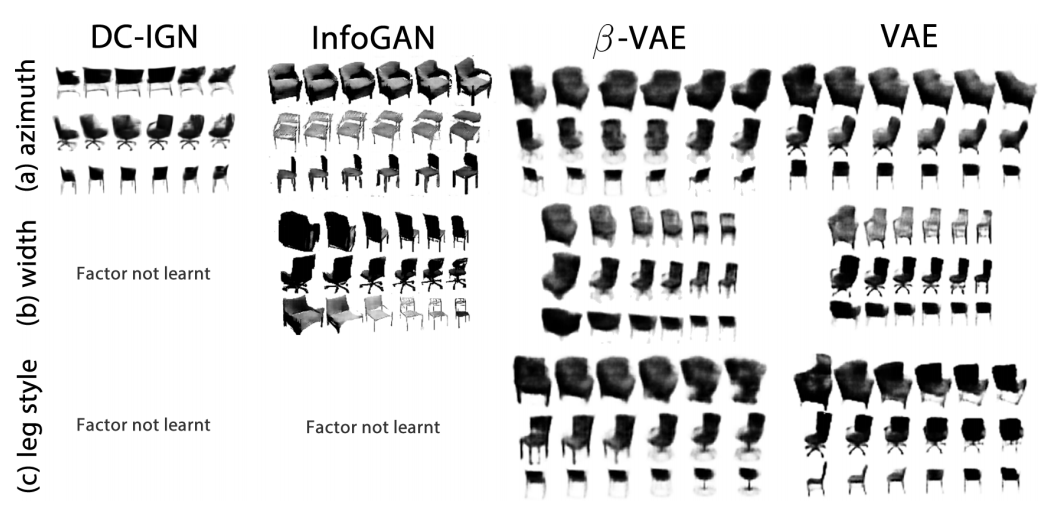
\includegraphics[width=1\textwidth]{imgs/3d_chairs.png}
                    \caption{Figures from \cite{higgins2016beta}. Qualitative comparison on disentanglement between DC-IGN\citep{kulkarni2015deep}, InfoGAN\citep{chen2016infogan}, $\beta$-VAE\citep{higgins2016beta}, and VAE\citep{kingma2014adam} on 3D images of chairs.}
                \end{figure}  
                
                \begin{figure}[H] \label{fig:3d_faces}
                    \centering
                    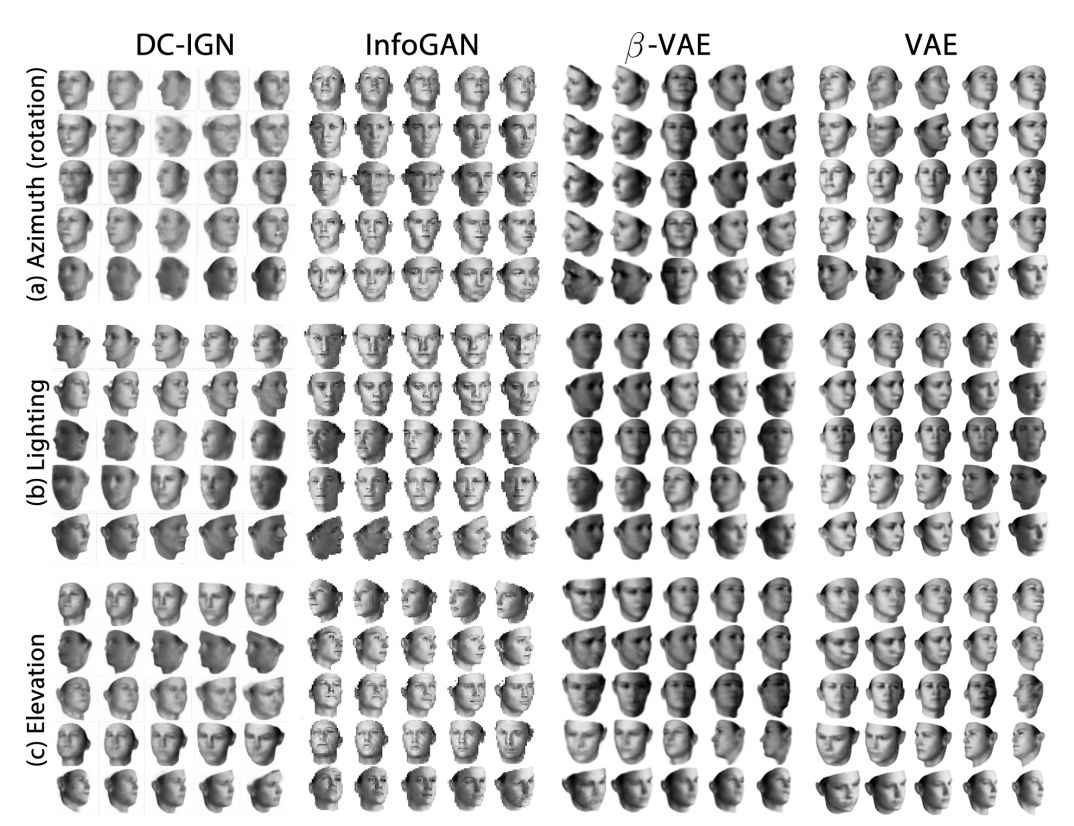
\includegraphics[width=1\textwidth]{imgs/3d_faces.png}
                    \caption{Figures from \cite{higgins2016beta}. Qualitative comparison on disentanglement between DC-IGN\citep{kulkarni2015deep}, InfoGAN\citep{chen2016infogan}, $\beta$-VAE\citep{higgins2016beta}, and VAE\citep{kingma2014adam} on 3d images of faces.}
                \end{figure}  
                
                What these figures are showing are various input images acting as the seed and varying the value of a single latent dimension to show the change in a single generative factor. As we can see from the result images, VAE already does a good job at mapping some generative factors to single latent dimensions which is what is required for disentanglement. However, we will see that in many ways, a more recent model called the $\beta$-VAE based on the standard VAE improves in disentanglement.
                
        \subsection{Beta-Variational Autoencoders($\beta$-VAE)}
            \subsubsection{Model description}
                \cite{higgins2016beta} introduced the $\beta$-VAE and the modification is very little from the original VAE. In fact, the only difference is the introduction of a single scalar $\beta$ as a hyperparameter in the original loss function. Recall that the loss function used in the original VAE is:
                
                \[ \text{Loss\textsubscript{VAE}} = \mathbb{E}_{q_{\bm{\theta_x}}(\bm{z}|\bm{x})} \left[\log p(\bm{x} | \bm{z}) \right] + KL\left[q_{\bm{\theta_x}}(\bm{z}|\bm{x}) || p(\bm{z})\right] \]
                
                The loss function for the $\beta$-VAE is:
                
                \[ \text{Loss\textsubscript{$\beta$-VAE}} = \mathbb{E}_{q_{\bm{\theta_x}}(\bm{z}|\bm{x})} \left[\log p(\bm{x} | \bm{z}) \right] + \textcolor{red}{\beta} KL\left[q_{\bm{\theta_x}}(\bm{z}|\bm{x}) || p(\bm{z})\right] \]
                
                By construction, $\beta=1$ gives the standard VAE but \cite{higgins2016beta} argues that the $\beta$-VAE, when $\beta>1$ improves disentanglement.
                
            \subsubsection{Intuitive reasoning of $\beta$-VAE}
                There is yet to be a formal argument as to why the presence of the $\beta$ term should improve disentanglement. However, the authors(\cite{higgins2016beta} and \cite{burgess2018understanding}) offers some intuitive reasoning. Firstly, recall that we can interpret the original VAE's loss function as:
                
                \[ \text{Loss\textsubscript{VAE}} = \text{Reconstruction Loss} + \text{KL Divergence} \]
                
                Then the $\beta$-VAE's loss function can be interpreted as:
                
                \[ \text{Loss\textsubscript{$\beta$-VAE}} = \text{Reconstruction Loss} + \textcolor{red}{\beta} \text{ KL Divergence} \]
                
                This makes the intent behind placing a scalar in front of the KL divergence clear enough. It is to be able to control the weight the KL divergence has on the total loss function. By increasing the value of $\beta$, the model will prioritise in trying to keep all the latent distributions as close to the standard Gaussian, the prior distribution. By decreasing the value of $\beta$, the model will prioritise in improving the reconstruction accuracy. 
                
    \section{Outline of project}
    
    \section{Motivation}
        \begin{itemize}
            \item Scope of this project(Unsupervised learning, Autoencoders, Disentangled latent space)
            \item like this
        \end{itemize}
        
